\documentclass[a4paper]{article} %
\usepackage{amssymb} %
\usepackage{setspace}
\usepackage{pslatex,palatino,avant,graphicx,color}
\usepackage{indentfirst}
\usepackage{enumitem}
\usepackage{setspace}
\usepackage{fancyhdr}
\usepackage[utf8]{inputenc}
\usepackage{listings}
\usepackage{color}
\usepackage{xcolor}
\usepackage[hidelinks,linkbordercolor=white,colorlinks=false]{hyperref}

\setcounter{tocdepth}{5}
\pagestyle{fancy}
\fancyhf{}
\renewcommand{\headrulewidth}{0pt}
\cfoot{\thepage}

\definecolor{mygreen}{rgb}{0,0.6,0}
\definecolor{mygray}{rgb}{0.5,0.5,0.5}
\definecolor{mymauve}{rgb}{0.58,0,0.82}

\lstset{ %
  backgroundcolor=\color{white},   % choose the background color; you must add \usepackage{color} or \usepackage{xcolor}
  basicstyle=\footnotesize,        % the size of the fonts that are used for the code
  breakatwhitespace=false,         % sets if automatic breaks should only happen at whitespace
  breaklines=true,                 % sets automatic line breaking
  captionpos=b,                    % sets the caption-position to bottom
  commentstyle=\color{mygreen},    % comment style
  deletekeywords={...},            % if you want to delete keywords from the given language
  escapeinside={\%*}{*)},          % if you want to add LaTeX within your code
  extendedchars=true,              % lets you use non-ASCII characters; for 8-bits encodings only, does not work with UTF-8
  frame=single,                    % adds a frame around the code
  keepspaces=true,                 % keeps spaces in text, useful for keeping indentation of code (possibly needs columns=flexible)
  keywordstyle=\color{blue},       % keyword style
  language=Python,                 % the language of the code
  otherkeywords={*,...},            % if you want to add more keywords to the set
  numbers=left,                    % where to put the line-numbers; possible values are (none, left, right)
  numbersep=5pt,                   % how far the line-numbers are from the code
  numberstyle=\tiny\color{mygray}, % the style that is used for the line-numbers
  rulecolor=\color{white},         % if not set, the frame-color may be changed on line-breaks within not-black text (e.g. comments (green here))
  showspaces=false,                % show spaces everywhere adding particular underscores; it overrides 'showstringspaces'
  showstringspaces=false,          % underline spaces within strings only
  showtabs=false,                  % show tabs within strings adding particular underscores
  stepnumber=2,                    % the step between two line-numbers. If it's 1, each line will be numbered
  stringstyle=\color{mymauve},     % string literal style
  tabsize=2,                       % sets default tabsize to 2 spaces
  title=\lstname                   % show the filename of files included with \lstinputlisting; also try caption instead of title
}

\lstset{ %
  backgroundcolor=\color{white},   % choose the background color; you must add \usepackage{color} or \usepackage{xcolor}
  basicstyle=\footnotesize,        % the size of the fonts that are used for the code
  breakatwhitespace=false,         % sets if automatic breaks should only happen at whitespace
  breaklines=true,                 % sets automatic line breaking
  captionpos=b,                    % sets the caption-position to bottom
  commentstyle=\color{mygreen},    % comment style
  deletekeywords={...},            % if you want to delete keywords from the given language
  escapeinside={\%*}{*)},          % if you want to add LaTeX within your code
  extendedchars=true,              % lets you use non-ASCII characters; for 8-bits encodings only, does not work with UTF-8
  frame=single,                    % adds a frame around the code
  keepspaces=true,                 % keeps spaces in text, useful for keeping indentation of code (possibly needs columns=flexible)
  keywordstyle=\color{blue},       % keyword style
  language=Java,                 % the language of the code
  otherkeywords={*,...},            % if you want to add more keywords to the set
  numbers=left,                    % where to put the line-numbers; possible values are (none, left, right)
  numbersep=5pt,                   % how far the line-numbers are from the code
  numberstyle=\tiny\color{mygray}, % the style that is used for the line-numbers
  rulecolor=\color{white},         % if not set, the frame-color may be changed on line-breaks within not-black text (e.g. comments (green here))
  showspaces=false,                % show spaces everywhere adding particular underscores; it overrides 'showstringspaces'
  showstringspaces=false,          % underline spaces within strings only
  showtabs=false,                  % show tabs within strings adding particular underscores
  stepnumber=2,                    % the step between two line-numbers. If it's 1, each line will be numbered
  stringstyle=\color{mymauve},     % string literal style
  tabsize=2,                       % sets default tabsize to 2 spaces
  title=\lstname                   % show the filename of files included with \lstinputlisting; also try caption instead of title
}

% Type down your paper title

\title{ChalkBoard: The Story of Font Packs}
% Authors
\author{Justin Brown, Dzu Pham, Jacob Drilling, Billy Rhoades, Sam Pilla \\ %
       Missouri University of Science and Technology %
       }%

\date{} 

\linespread{2.25}

\textwidth=15cm \hoffset=-1.2cm
\textheight=25cm \voffset=-2cm 

\setlist[itemize]{itemsep=-8pt, itemindent=0pt, leftmargin=*}



% Type down your paper title
\title{\vspace{30mm}ChalkBoard: The Story of Font Packs}

% Authors
\author{Justin Brown, Dzu Pham, Jacob Drilling, Billy Rhoades, Sam Pilla \\%
       Missouri University of Science and Technology%
       }%

\begin{document}

\maketitle

\pagebreak

\tableofcontents

\pagebreak

\setlength\parindent{0pt}

% The abstract

\begin{abstract}

This report contains the methods and models of execution for developing the Android application ChalkBoard. Using SCRUM, we developed the software over the course of 5 weeks. We began by designing an outline for the application, one that would keep track of assignments for classes and their grades. We then created a GitHub repository so that, outside of SCRUM meetings, we could monitor progress and be able to revert changes if a step in the development of the software was broken.

\end{abstract}

\section{Introduction}

College students are always on the move, whether it be from home to school, activity to project, or homework to sleep. They need something to easily keep track of their academics. We created that tool for them, a simple and elegant application, Chalkboard, that they can have with them when they are on the move.


Chalkboard is a mobile Android application that allows a user to keep track of their classes while also being able to calculate the individual grades of each of their classes. The application gives the user the option to store homeworks, projects, exams, labs, etc. into different categories. The user can then weight each category in accordance with the instructors weighting to show how each assignment affects their grade and provide a fully accurate measure of their overall grade. 

To develop Chalkboard, the team employed the SCRUM software development model. This agile model was chosen as it would keep the group focused on the project. It was also chosen as it provided flexiblity in the requirements of the application. We were able to start quickly with our first sprint; prioritizing the basic functionality of the application. We then used the period after the first sprint to evaluate the time constraint and our personal requirements of the application.
\section{Implementation}

\centerline{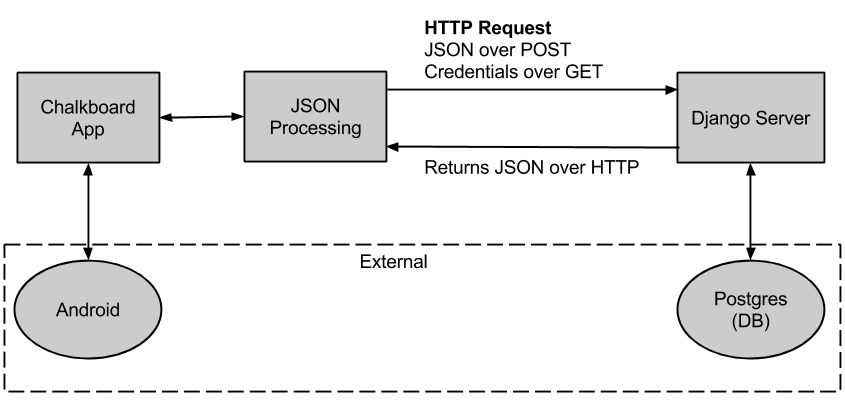
\includegraphics[scale=.5]{design.png}}

\subsection{PostgreSQL}

After the second sprint, PostgreSQL was selected as a database backend over SQLite due to performance constraints. The schema for PostgreSQL was autogenerated from Django-provided models, which can be found in Section \ref{Django Models}. Choosing Django to manage PostgreSQL for us allowed us to change schema on the fly without losing data. For example, in Section \ref{First Sprint Third Scrum} we changed weight to be per homework to per category. Instead of having to purge the database contents and redo our schema, we simply performed a migration.

\subsection{Django/API}

Django was selected due to, as mentioned above, its ability to abstract database management away into objects. Easy database changes, database handling with no queries, and methods which allow API calls to simply be one method.  Django is a web framework which is used as a library in Python. Our usage of Django was as a web API.
Queries were made to a URL. For example, a query to add a course would go to:

\indent\url{http://cs3100.brod.es:3100/add/course/}

All URLs have to be authenticated in order to go through. A token is obtained from the following URL by sending it your username and password in JSON via POST:

\indent\url{http://cs3100.brod.es:3100/token/get.json}

This then returns a token and a userid, this is passed to every call on the URL. For example, to add a category, call:

\indent\url{http://cs3100.brod.es:3100/add/grade/?user=4&token=34y-10ca4d90c5d6e031e3}

JSON is sent up which contains information for each individual call. Here are the calls that are supported:

\begin{itemize}
  \item /add/%
    \begin{itemize}
      \item grade/
        \item category/
        \item course/
        \item homework/
    \end{itemize}
    \item /get/%
    \begin{itemize}
      \item grade/
        \item category/
        \item course/
        \item homework/
    \end{itemize}
    \item /edit/%
    \begin{itemize}
      \item grade/
        \item category/
        \item course/
        \item homework/
    \end{itemize}
    \item /course2cat/
    \item /rm/grade/
\end{itemize}

Django abstracts most of these calls into less than 300 lines written by our team. The remove calls were only allowed on grades due to referential constraints between all of the other models. The course2cat was a modification added in late in the project. Course2cat returns a list of all courses which use a category.

\subsection{Java/Django Communication}

When it was decided Django would be used as the backend server, it meant there would have to be communication with Django and the backend Java, sending and receiving both ways. In order to do this efficiently, we used a JSONObject library and the built in HTTP library for Java. The JSONObject library could convert to and from Strings, allowing a lot of versatility for receiving and returning variables for communicating with Django. The HTTP library allowed us to contact the Django server and send it the JSON it needed to add, modify, or delete data. 

The actual implementation involved a few varying functions since Django needed different JSON for different functionality. For reading, adding, editing, and removing, the functions would receive the user ID, token, what category the data is under (course, grade, etc.), and the JSON query for what Django will read, add, remove, or edit. In order to authenticate a user, the function would be passed the username and password, then pass those onto Django to compare them to what the server has saved, ensuring the login information is valid.

Originally, registration went through these Java functions. It would accept a username, password, and email, pass those to the Django server through JSON, and Django would then add them to the database server. However, we decided it would be best to register through Django itself, and so these functions are not implemented.

All these functions are returned JSON with any data the need, such as access getting back the information it requested, and a return value of true or false. If true, the functions would then return success and any data as JSON to the Java backend. If false, the function would throw an exception. The Add function can be found in Section \ref{Jabba Code}.
\subsection{Java Backend}
The Java backend is comprised of a structure of four java classes: User, Course, WeightedGrades, and Assignment. The way these four classes interact to create the data structure can be seen in the UML Diagram below. A user has a username, an ID and token used to log in and access the database. Additionally the user has a list of courses. Each course has a list of Weighted Grades, which has a list of assignments. This structure provides incredible flexibility so that a user can add  as many courses, grade categories, or assigments as they desire. This also allows for different grading systems among the users many courses. Furthermore, this data structure made it very easy to pass all of the users data between views in the user interface.

The data structure itself loads from the JSON passed back from the DJango server.  Converting from JSON to the Java data structure is incredibly easy when using the JSONObject library. This load is done all at once when the user logs in, and the data is added to the database as the user adds it in the application. This gives a long initial load, but loading the individual pages is extremely fast. To decrease loading time, the data structure can loads on a thread seperate from the user interface. This threading allows the user interface to load and react smoothly even when the application is performing the long load from the database. To further decrease loading speed in the future, loading courses could be threaded seperately so that the user can interact with a class before all classes have completely loaded.

\centerline{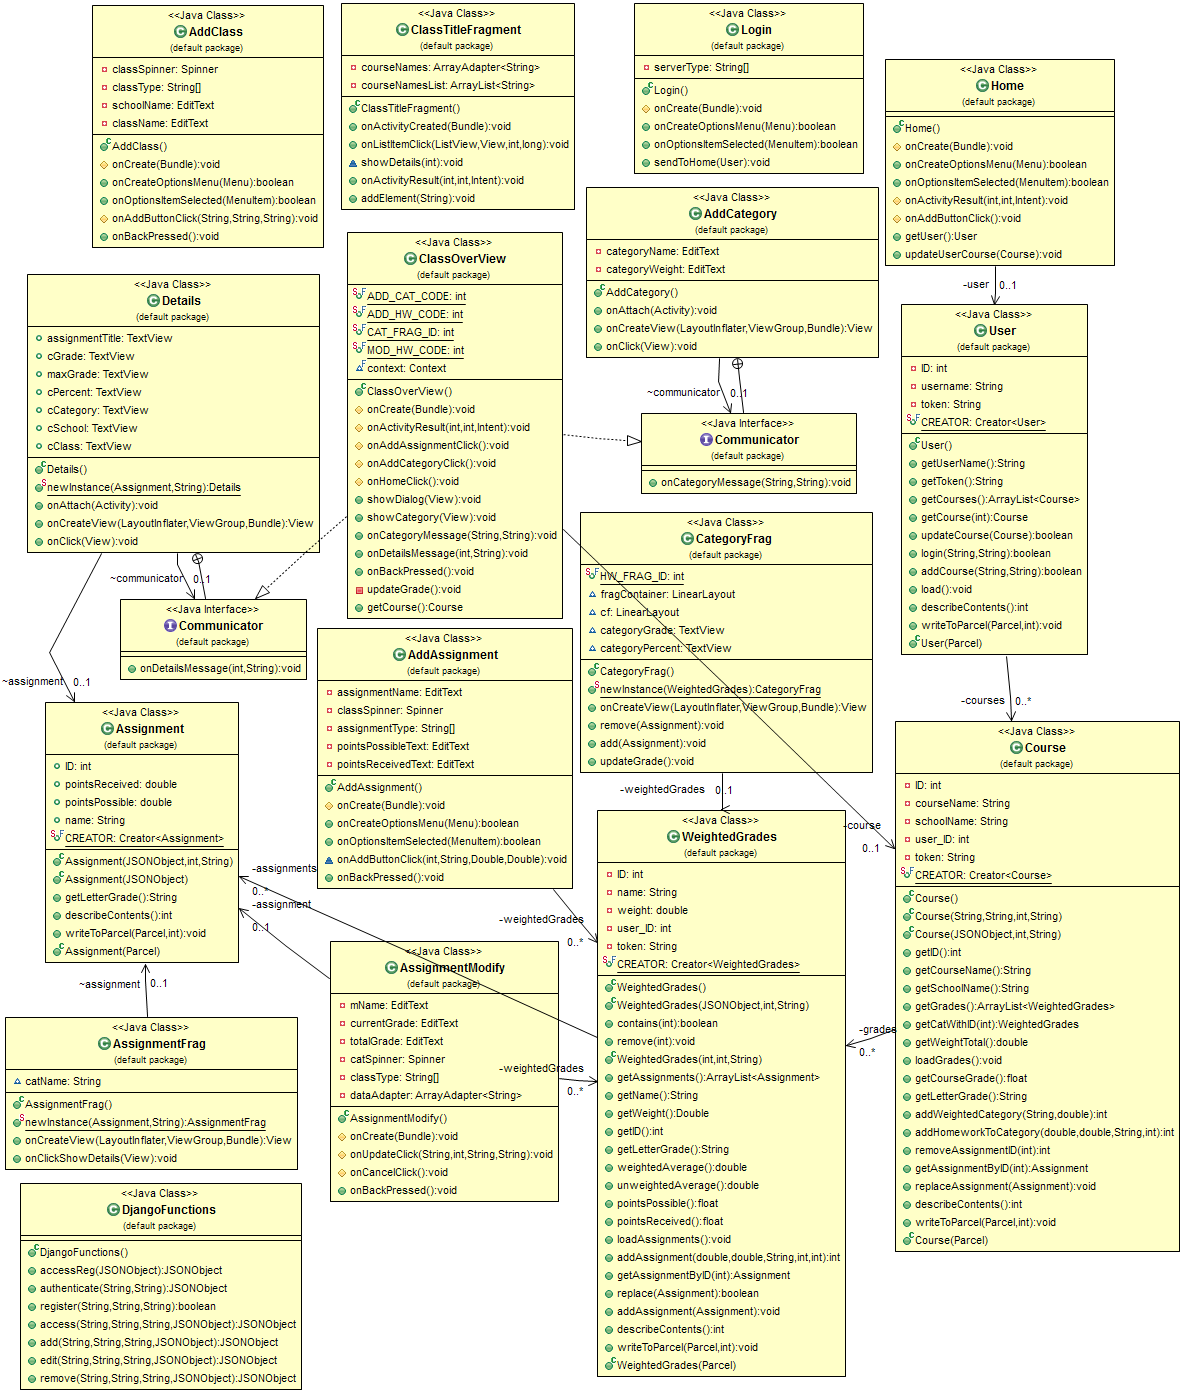
\includegraphics[scale=.45]{CS3100.png}}
This is our Unified Modeling Language diagram.

\subsection{Android Frontend}
For the front end, Android, as a platform, consists of XML and Java. The XML is used to create and manage the visuals of each layout. This includes creating the buttons, Text Views, the Edit Text boxes, the drop down menus, etc. The XML is also used to house strings, defined elements and the style references as well as manged how each element of the interface appears and interacts with the others on each page. Java is used to give the layouts functionality, such as the function when a button is pressed, switching layouts (screens) and sending data to other layouts, and giving the application dynamic capabilities. With Java we were able to create XML code to display new Text Views as classes were added, dynamically create and edit strings for use by the user and make the data persistent across layouts.

\textbf{Login page}:\\
The login page has little XML compared to the others. This page allowed a user to login and, if they did not already have an account, navigate to the sign up page and create an account. Using Java, mixed with the DJango server, we were able to incorporate login credential checking. To prevent users from returning to the login page and causing confusion, we have the login layout process destroy itself on when the new activity is called. 

\textbf{Home Page}:\\ 
The homepage contains an array list that would pull the class name from the table housed on the server and displays them as a clickable button. Having them as a clickable button gave a cleaner interface with a straightforward idea of how to navigate to individual class views. There is also an add class button located at the bottom of the page. Once it is clicked it will take the user to another page and display data from the server that is revelent to that class.

\textbf{Class Overview Page}:\\
We went through many design iterations for this page trying to get the content to be organized in a manner that was clear, made sense, and presented the pages functionality. We finally landed on a divider design that distinctly displayed each assignment in a visually appealing way. Each category is displayed as a header and bolded so it will stand out. Included in the header will be the letter grade and the total grade caculated from each assignment. Next to each of the individual assignment there will be a button that is named details. When this details button is clicked it will open up a dialog box that will display more information about the current assignment. Inside this dialog box it will give the user three options delete, modify, or return.

At the top of the class overview page contains three buttons; return home, add category, and add assignments. When the user first creates a class the user should create a category first. If the user tries to enter an assignment before they have a category created the app will throw up an alert dialog. This will inform the user that it is impossible to add and assignment before a category is created. Underneath the buttons contains the total grade of the class. This grade is calculate from the weighted grades from each of the category.


\textbf{Add/Delete/Modify}:\\
There are two different types of add pages; the add assignment and add class page. This will take the user into a different page were they are to fill out the required fields. Once the user is done and click the finish button then the data is sent to the server. On return to the previous page it will force a refresh and pull the updated data form the server.

The delete option will just set a function to the server and find the class or assignment name and remove all data conntected to that field. For the modify option it will pull the user into another page. This page contains empty fields and lets the user choose which field they want to modify. Fields that are left blanks are taken as unchanged data while fields that contains anything new will be updated on the server.


\section{First Sprint}

For this project we chose to floow the Scrum model and the first sprint meeting took place on <bla>. This meeting was short and mostly detailed what we wanted out of the project. Our initial goal was to design a product that we could use personally in our every day life and that other students could also benefit from. We had a total of three initial ideas. The two that had lost out were a rent keeping and payment reminder application and check/tip splitter. We decided against the rent keeper because we felt we would not use it frequently enough and we decided against the check/tip splitter because that would have incorporated using people's credit or debit cards and did not feel like we had time to implement that feature securely. After ruling those two ideas out, we loosely outlined requirements and decided on an idea to implement. A grade tracking program was selected by the group. 
\\
We set out to design a program which was:

\begin{itemize}
  \item On mobile or other high-accessibility platform
    \item A tool that was useful to us
    \item Centralized server for user data access
    \item Secure user authentication system
\end{itemize}

Functional constraints were also decided. A user should be able to add a grade in under 10 seconds to a course, barring other setup requirements. Additionally, our sprint cycle was set at 5 weeks, with a second short cycle for a week. Our scrum meetings were planned every four days provided everyone could meet. Finally the teams were decided as follows: \\
 
\textbf{Backend}:  Jacob Drilling, Sam Pilla, Billy Rhoades\\
\textbf{UI}:  Dzu Pham, Justin Brown \\

The teams for the backend and the user interface were chosen based on a combination of volunteering to learn a particular aspect of working with an android application, the preference to work on a particular portion and the opportunity to apply current skills to a new project. Additionally, Billy was designated as Scrum master by the group. Throughout the process, Billy led meetings, organized meeting minutes, and made sure the teams were completing their tasks.
\\

Tasks for each team were also decided and delegated:

\textbf{Backend}:
\begin{itemize}
  \item Create database schema
    \item Implement database schema in Django
    \item Create basic data structure for transactions in Android
    \item Accessor functions for the database in Android
% * <sjpn96@mst.edu> 2015-05-08T00:18:39.043Z:
%
% 
%
% * <sjpn96@mst.edu> 2015-05-08T00:18:35.673Z:
%
% 
%
\end{itemize}

\textbf{Frontend}:
\begin{itemize}
  \item Design application icon
  \item Create login page
    \item Create overview page
    \item Create addClass page
\end{itemize}


\subsection{First Scrum}

The second meeting, and first scrum, took place on 4/8/15. All group members were present. This meeting consisted mostly of demoing progress and outling future issues.

Presentables:
\begin{itemize}
  \item Jacob brought a schema for the database
    \item Justin brought a basic app implemented in Android
\end{itemize}
%
% <INSERT REFERNECE TO SCHEMA APPENDIX> %
% Schema is available on gdocs
%

\centerline{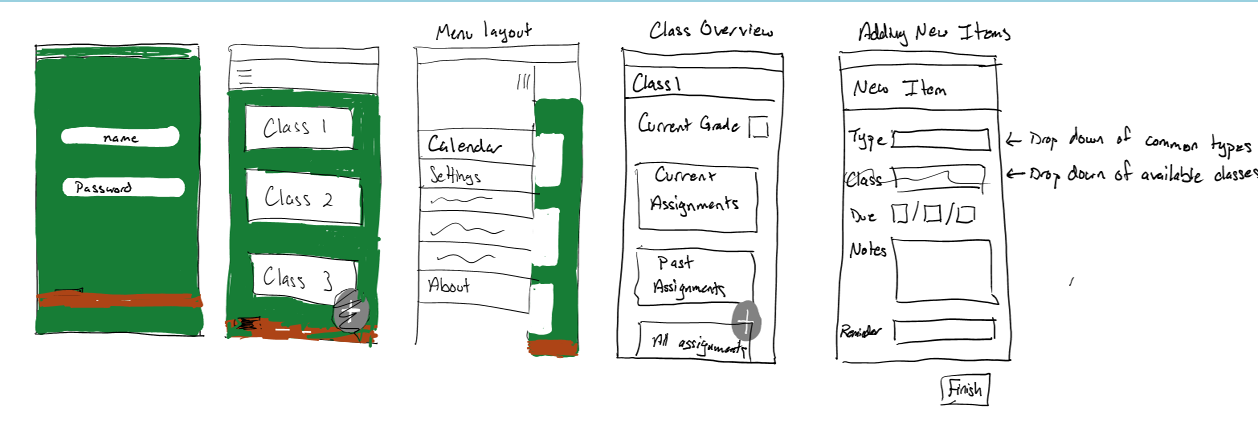
\includegraphics[scale=.75]{Picture1.png}}

During this meeting version control methods were also decided and implemented. Additionally, we decided on a target Android version, 4.0 ICS API 15, because we felt it encompassed a large enough percentage of current Android phones on the market. \\

\subsection{Second Scrum}

The second scrum took place on 4/15/15. Due to Spring Break, this scrum was offset by a week. During this meeting modules from individual teams begun to integrate. We really started getting in to connecting the backend to the user interface. The modules we connected at this time were the login page to the server that was to house a users login credentials. We then began working with the overall API's for both the Android application and the DJango driven server. \\

Presentables:
\begin{itemize}
  \item Django API was added for getting and adding elements
    \item Basic API accessing was started for the Android app
\end{itemize}

%
% <Show Django API basics, doc?>
%

\subsection{Third Scrum} \label{First Sprint Third Scrum}

The third scrum took place on 4/20/14. This scrum meeting all but concluded the first sprint cycle. This meeting contained the first prototype for our application. This prototype had very basic functionality. The application could display the users data and contained functionality to add courses, categories, and grades.

Presentables:
\begin{itemize}
  \item Moved weight in the schema to category
    \item Implemented the registration API
    \item Fully documented Django API
    \item Sam and Jacob showed prototype Java API interface
\end{itemize}

\section{Second Sprint}

The second sprint was marked by division of effort. Roughly half of the application had been put down, with a little more than half remaining. The first sprint's conclusion was marked by the basic add, get, and display implementation within the application by both frontend and backend teams. Additionally, the team collectively agreed to implement more functionality to complete the interface. This sprint cycle was shorter than the first, so meetings were more frequent. This included:

\begin{itemize}
  \item Modification of all tables (courses, grades, categories, homeworks)
    \item Deletion of grades\\
\end{itemize}

The tasks for the second sprint were as follows: 

\textbf{Backend}:
\begin{itemize}
  \item Modification of tables through API
    \item Polishing accessing in Java
    \item Deletion of grades through API
    \item Clean error handling to pass to UI
\end{itemize}

\textbf{Frontend}:
\begin{itemize}
  \item User-friendly errors
    \item Backend integration
    \item Interface details: box for additional information, prefilled categories, toasts
    \item Dynamic table for category integration
    \item Modification page and handling
    \item Deletion button
\end{itemize}

\subsection{First Scrum}

The first scrum of the second sprint cycle occured on 4/22/15. This meeting was short, and consisted of brief discussion over the progress of current tasks.

Presentables: 

\begin{itemize}
  \item Sam completed Android backend support for add, register, and get 
    \item Java data structure for Android backend finished
    \item Homepage class array completed
\end{itemize}

\subsection{Second Scrum}

This scrum session was when the back end data was able to be visualize on the front end. Homepage was able to display the different classes and go to the appropriate class over page. From the class over view page we were able to pull the data for each category and display the following assignments. 

%Jacob & Dzu

4/24/15

Presentables: 

\begin{itemize}
  \item Completed frontend and backend integration
    \item Spruce up the interface
    \item Added return button
    \item Optimize user login and display data
\end{itemize}

\subsection{Third Scrum}

This scrum session consisted of integration between API and backend, backend with frontend. It included full implementation of modification and deletion. Testing was mostly done this day as well, as a mock demo was conducted with the entire team. 

4/26/15

% Met at Justin's

Presentables: 

\begin{itemize}
  \item Implemented deletion for grades for API
    \item Implemented modification for all tables for API
    \item Migrated for SQLite to PostgreSQL
    \item Further debugging with Java API accessors
\end{itemize}

\section{Testing}
Testing was done after developers completed each task and also at the conlcusion of each sprint. White box unit testing and input boundry testing was performed after each task was completed. For example, unit testing on the database was performed using a Chrome application called postman. This application allowed us to test each query individually, independent of the application. One crucial bug discovered at this stage was the database not storing the points possible for any homework. Input boundry testing also found a bug where some names would crash the front end applicaiton.

Most of the testing performed on the application was black box testing at the conclusion of the second sprint cycle. This was because we were new to android developement and, therefore, we thought most of the bugs would happen when integrating the back end. Our prediction was correct and it was during this testing that the majority of the bugs were found. During the integration and system testing, we tested the functionality of the application as a whole, such as adding, deleting, and modifing grades. We also tested malicious input to make sure the system was secure. More specific testing results are listed in \ref{Testing Results}

\section{Future}
When we were initially generating ideas, we came up with many features that could not feasibly be done in the time frame we were given. One feature that could be implemented in the future is adding 'instructor accounts.'  With this feature, instructors could create courses and add users(students) to the course. Then the instructor would be the only person allowed to add or change grades. This feature, if implemented, could be made optional and users would still be able to add classes independently.
\\
Another feature that could be added is the ability for a student to predict their grade. Many students keep grades so that they can decide what grade they need on a test or a final exam to keep their current letter grade. This feature would allow students to enter a desired final grade, and the app would predict the score needed to achieve that final grade. The team wanted to implement this feature originally, but it was not included the first two sprint cycles. The team decided it was of a lower priority when compared to add, delete, and modify functionality.
\\
We had such a clever and fun font, so we thought: why not give the user the option to change the font to better suit their preferences? This is how we came up with the idea to potentially include font packs. This would also become a potential source of income. Another source of income would be to incorporate ads into our application. These would be directed towards students but would enable us upgrade the server, or even get paid.


\section{Appendix}

Full source code can be found at: https://github.com/ArthurSemilla/cs3100

\subsection{Burn Down Chart} \label{Burn}
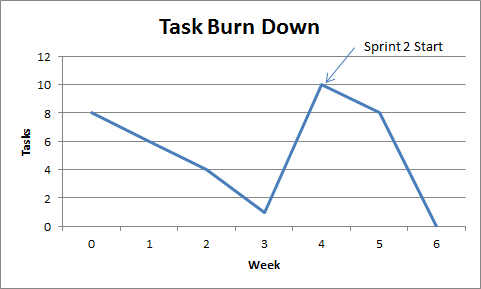
\includegraphics[scale=0.75]{BurnDown.png}

\subsection{Testing Results} \label{Testing Results}
\begin{enumerate}
  \item Got a working prototype
  \begin{itemize}
    \item No working functionalities
        \item The app was stable, everything was working as expected
  \end{itemize}
  \item Backend server was created
    \begin{itemize}
    \item Login worked as expected
        \item Data tables were getting filled correctly
        \item Loading data was not as optimal as we hoped (there were many methods for doing the same thing)
  \end{itemize}
    \item Front end and Back end intergration 
    \begin{itemize}
    \item App would crash because fragments were not getting called correctly
        \item There was a problem with XML not rendering the dynamic templates correctly
        \item The layout was disoriented when trying to add boarders
        \item Sometime the app would crash if a certian process was excuted
        \begin{itemize}
      \item For example: After the user enters in an assignment and then returns to the home page the app crashes
    \end{itemize}
        \item The return button was not closing the curren activity correctly
  \end{itemize}
    \item Final testing: Migrated over from SQLite to PostgreSQL
    \begin{itemize}
      \item Optimize the loading of the data tables
        \item Patched up small bugs
        \item Kept improving UI aspects to remove glitches
    \end{itemize}
\end{enumerate}

\subsection{Django Models} \label{Django Models} \linespread{1}

\begin{lstlisting}[language=Python]
from django.db import models
from django.contrib.auth.models import User

class Category( models.Model ):
    name = models.CharField( max_length=100 )
    weight = models.FloatField( default=1 )

class Course( models.Model ):
    school = models.CharField( max_length=255 )
    name = models.CharField( max_length=100 )

class Homework( models.Model ):
    category = models.ForeignKey( Category )
    name = models.CharField( max_length=100 )

    points_possible = models.FloatField( default=0 )

class Grade( models.Model ):
    course = models.ForeignKey( Course )
    user = models.ForeignKey( User )
    homework = models.ForeignKey( Homework )
    
    points_received = models.FloatField( default=0 )
\end{lstlisting}

\pagebreak
\subsection{Add Function for Java/Django Communication} \label{Jabba Code}
\begin{lstlisting}[language=Java]
public JSONObject add(final String dataToAdd, final String userID, final String token, JSONObject query)
{
    String urlString = "http://cs3100.brod.es:3100/add/" + dataToAdd + "/?user=" + userID + "&token=" + token;
    JSONObject returnJSON = null;

    try
    {
        //HTTP code to contact the Django server and send it the JSON to register
        HttpClient httpclient = new DefaultHttpClient();
        HttpPost httppost = new HttpPost(urlString);

        //passes the Django server the JSON for registration
        StringEntity regString = new StringEntity(query.toString());
        httppost.addHeader("content-type", "application/x-www-form-urlencoded");
        httppost.setEntity(regString);

        HttpResponse response = httpclient.execute(httppost);

        //return string from Django server
        HttpEntity httpEntity = response.getEntity();
        String resultString = EntityUtils.toString(httpEntity);

        returnJSON = new JSONObject(resultString);
    }
    catch(Exception e)
    {
        e.printStackTrace();
    }
    return returnJSON;
}
\end{lstlisting}

\subsection{XML layout}
\begin{lstlisting}[language=XML] 
//These are the basic layout on how to display something in XML
//This specific code creates the assignment in the list and gives it a button
<LinearLayout android:id="@+id/lay9"
  android:layout_width="fill_parent"
  android:layout_height="wrap_content"
  android:orientation="horizontal">

  <TextView  android:id="@+id/assignmentTitle"
        android:layout_width="0dp"
        android:layout_height="wrap_content"
        android:textColor="@color/white"
        android:layout_weight="2"
        android:text="Homework"/>

  <TextView android:id="@+id/assignmentGrade"
        android:layout_width="0dp"
        android:layout_height="wrap_content"
        android:gravity="center_horizontal"
        android:textColor="@color/white"
        android:layout_weight="1"
        android:text="A"/>

  <Button android:id="@+id/assignmentDetails"
        android:layout_width="0dp"
        android:layout_height="wrap_content"
        style="?android:attr/borderlessButtonStyle"
        android:textColor="@color/white"
        class="rsck.chalkboard.AssignmentFrag"
        android:layout_weight="1"
        android:text="Details"/>

</LinearLayout>
\end{lstlisting}
\end{document}
